%
% Adapted from File acl-hlt2011.tex
%
% Contact: gdzhou@suda.edu.cn
%%
%% Based on the style files for ACL2008 by Joakim Nivre and Noah Smith
%% and that of ACL2010 by Jing-Shin Chang and Philipp Koehn


\documentclass[11pt]{article}
\usepackage{acl-hlt2011}
\usepackage{times}
\usepackage{latexsym}
\usepackage{amsmath}
\usepackage{multirow}
\usepackage{url}
\usepackage{graphicx}
%\DeclareMathOperator*{\argmax}{arg\,max}
%\setlength\titlebox{6.5cm}    % Expanding the titlebox
\setlength\titlebox{3.5cm}    % Expanding the titlebox

\newcommand{\mnote}[1]{\marginpar{\raggedleft\footnotesize\itshape#1}} 

\title{Paraphrase Acquisition Combining Monolingual and Bilingual Information}

%\author{First Author \\
%  Affiliation / Address line 1 \\
%  Affiliation / Address line 2 \\
%  Affiliation / Address line 3 \\
%  {\tt email@domain} \\\And
%  Second Author \\
%  Affiliation / Address line 1 \\
%  Affiliation / Address line 2 \\
%  Affiliation / Address line 3 \\
%  {\tt email@domain} \\}

\date{}

\begin{document}
\maketitle
\begin{abstract}
This paper improves an existing bilingual paraphrase extraction technique using monolingual distributional similarity to re-rank candidate paraphrases.  Raw monolingual data  provides a complementary and orthogonal source of information that lessens the commonly observed errors in bilingual pivot-based methods. We incorporated a newly developed locality sensitive hashing algorithm into the monolingual score calculation in order to facilitate a practical implementation of this method over large volumes of data. Preliminary evaluation demonstrates that monolingual scoring of bilingually extracted paraphrases has a substantially stronger correlation with human judgment than the probabilities assigned by the bilingual pivoting method. test

%This shows promises in further improvement of paraphrase quality through merging of the variety of scores...@@

\end{abstract} 


\section{Introduction}
\mnote{add back some details that were omitted due to acl short ppr constaint?}
Paraphrases are the rewording of a phrase in which the meaning is preserved. Data-driven paraphrase acquisition techniques can be categorized by the type of data that they use \cite{MadnaniDorr10}.  Monolingual paraphrasing techniques cluster phrases through statistical characteristics such as dependency path similarities or distributional co-occurrence information \cite{Lin01discoveryof,PascaDienes05}.   Bilingual paraphrasing techniques use parallel corpora extract potential paraphrases by grouping English phrases that share the same foreign translations \cite{BannardCallisonBurch05}.  Other efforts blur the lines between the two, applying techniques from statistical machine translation to monolingual data or extracting paraphrases from multiple English translations of the same foreign text \cite{Barzilay2001,PangEtAl03,QuirkDolanBrockett04}.

%Although the knowledge used by monolingual and bilingual paraphrasing techniques is largely orthogonal, only limited effort has been devoted to merging the two lines of work to develop new methodologies and applications. For instance, word-alignment from parallel monolingual data was used to train a phrasal ``translation" model \cite{QuirkDolanBrockett04}; paraphrases extracted from output of SMT trained on bilingual text are incorporated into query expansion for answer retrieval \cite{RiezlerEtAl07}.

%@@ include additional applications?@@
%Additional application of paraphrases in the domain of natural language processing includes text summarization (McKeown et al., 2002), headline or title generation (Dorr et al., 2003; Vandeghinste and Pan, 2004; Marsi et al., 2009,),  Recently paraphrase models has also been considered for sentence compression (?courtney's). An extensive survey of paraphrase methods is contained in \newcite{MadnaniDorr10}.

We exploit both types of data, applying a monolingually-derived similarity metric to the output of the pivot-based bilingual paraphrase model.  In this paper we:
\begin{itemize}
\item Show that monolingual cosine similarity calculated on large volumes texts ranks bilingually extracted paraphrases better than the paraphrase probability originally defined by \newcite{BannardCallisonBurch05}
\item Scale to very large sets of candidate paraphrases using locality sensitive hashing and online signature generation \cite{Charikar02,VanDurmeLallACL10}
\item Something else
\end{itemize}
% Our work overlaps with their approach in the paraphrase generation with bilingual translation rules. However, instead of assigning paraphrase score based on phrase translation probabilities, we introduced a measure dependent on monolingual distributional similarity built upon large n-gram corpus. Locality sensitive hashing method of \newcite{Charikar02}, which has been recently extended to online signature generation by \newcite{VanDurmeLallACL10}, was implemented to enable faster computation by reducing the similarity feature space dimension with random projection. Descriptions on each stage of the process will be covered in the following sections, which are followed by examples and evaluation results.

%@@ previous work on paraphrasing reranking (monolingual and bilingual based?) @@


%\section{Related Work}
%@@ previous work on paraphrasing (monolingual and bilingual based); @@
%One example is the work on discovery of inference rule, analogous to paraphrasing, with parsed dependency trees  
%@@ Nitin Madnani's survey ppr on data driven paraphrase methods@@
%


%\section{Multilingual Paraphrase Extraction via Pivoting}
\section{Related Work}

 \newcite{BannardCallisonBurch05} proposed identifying paraphrases by pivoting through phrases in a bilingual parallel corpora. 
Figure~\ref{paraphrase-illustration} illustrates their paraphrase extraction process. A phrase to be paraphrased, like {\it thrown into jail}, is found in a German-English parallel corpus.  The corresponding foreign phrase ({\it festgenommen}) is identified using word alignment and phrase extraction techniques from phrase-based statistical machine translation \cite{KoehnEtAl03}.  Other occurrences of the foreign phrase in the parallel corpus may align to another English phrases like {\it jailed}.  %Following \newcite{BannardCallisonBurch05}, we treated any English phrases that share a common foreign phrase as potential paraphrases of each other.
%
As the original phrase occurs several times and aligns with many different foreign phrases, each of these may align to a variety of other English paraphrases.  Thus, {\it thrown into jail} not only paraphrases as {\it jailed}, but also as {\it arrested}, {\it detained}, {\it imprisoned}, {\it incarcerated}, {\it locked up}, and so on.
%{\it taken into custody}, and {\it thrown into prison} and others like {\it be thrown in prison}, {\it been thrown into jail}, {\it being arrested}, {\it in jail}, {\it in prison}, {\it put in prison for}, {\it were thrown into jail}, and {\it who are held in detention}. 
Bad paraphrases, such as
 {\it maltreated}, {\it thrown}, {\it cases}, {\it custody}, {\it arrest}, and {\it protection}, may also arise due to poor word alignment quality and other factors.

\newcite{BannardCallisonBurch05} defined a paraphrase probability to rank these paraphrase candidates,  as follows:
\begin{eqnarray} \label{paraphrase-prob-1}
 \hat{e_2}	& = & \arg \max_{e_2 \neq e_1} p(e_2 | e_1)\label{paraphrase-prob}  \\
  p(e_2|e_1) &=& \sum_f p(e_2,f|e_1)\\
                  &=& \sum_f p(e_2|f,e_1) p(f|e_1) \\
                  &\approx& \sum_f p(e_2|f) p(f|e_1)
\label{paraphrase_prob_eqn}
\end{eqnarray}
where ${p(e_2|e_1)}$ is the paraphrase probability, ${p(e|f)}$ and ${p(f|e)}$ are the translation probabilities from a statistical translation model.  

Anecdotally, this paraphrase probability sometimes seem unable discriminate between good and bad paraphrases, so some researchers disregard it and treat the extracted paraphrases as an unsorted set \cite{Snover2010}.  \newcite{CallisonBurch08} attempts to improve the ranking by limiting paraphrases to be the same syntactic type.  

We attempt to re-rank the paraphrases using other information.  This is similar to the efforts of \newcite{ZhaoEtAlACL08}, who ...



\begin{figure}
\begin{center}
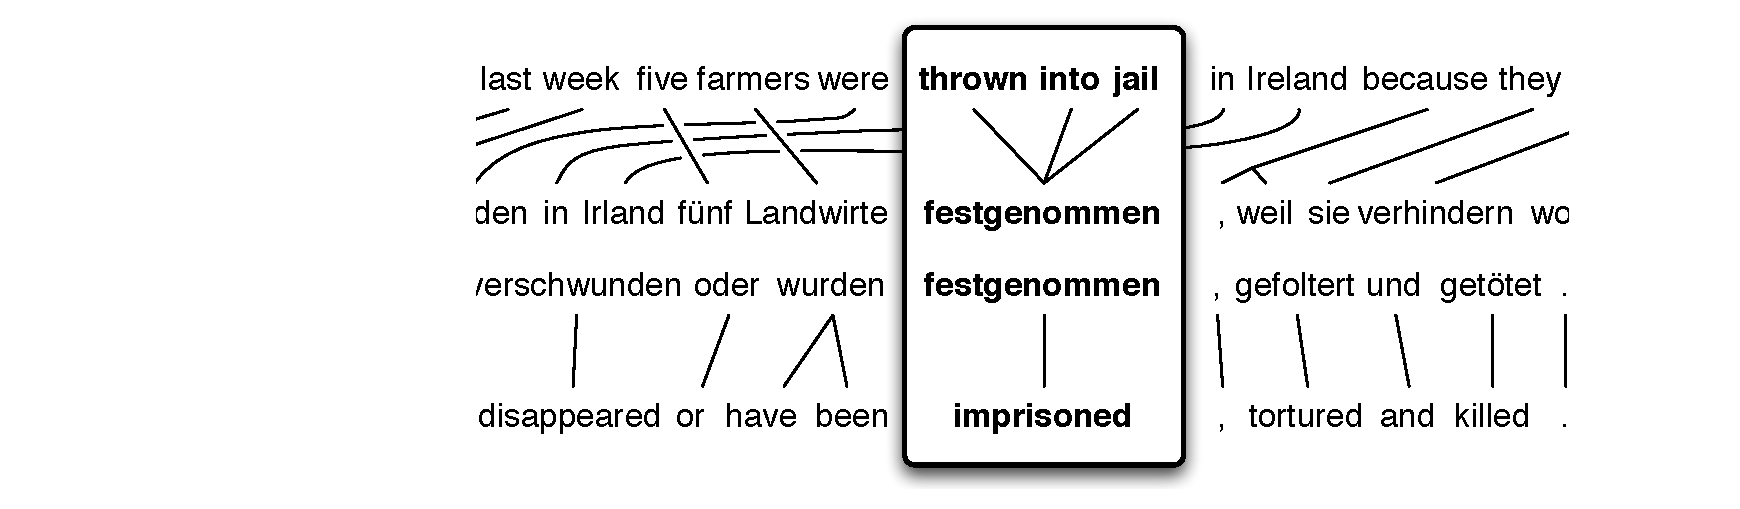
\includegraphics[width=\linewidth]{pivot-2}
\end{center}
\caption{\small Using a bilingual parallel corpus to extract paraphrases.}
\label{paraphrase-illustration}
\end{figure}

%\section{Confidence Measure based on Monolingual Distributional Similarity}
\section{Using Monolingual Resources}
\label{sect:mds}

\mnote{ insert summary on Monolingual Distributional Similarity }

\section{Dimensionality Reduction via LSH}
\label{sect:lsh}

\mnote{ insert LSH summary }


\section{Evaluation}
We evaluate the paraphrase confidence metrics by first demonstrating through some paraphrase examples the characteristics of each ranking method. Next we present the results from a pilot study conducted for text summarization based on human judgments to draw qualitative comparison between different metrics. Results from the pilots study led to a larger scale evaluation of the re-ranking methods based on paraphrase extraction pivoting through the French-English corpora, of which the details and observations are discussed in the last sub-section.

\subsection{Data and Metric}
@@ include this section if ur-en mTurk result produces reasonable 
@@ explain Kendall Tau and Kendall Tau b

\subsection{Paraphrase Examples}

@@ no mTurk results, show only few examples to motivate study, emphasize of "low-resource"-pivoting @@

A bilingual paraphrase model was trained using the parallel corpus between Urdu and English from NIST 2009. The model for both the original pivoting-based method in \newcite{BannardCallisonBurch05} and the syntactically constrained (S-C) method in \newcite{CallisonBurch08} were constructed with a grammar extractor based on SAMT formalism developed by \newcite{ZollmannVenygopal06}. The data set, which was collected from newswire and weblogs, consists of roughly 1.7 million words and 200K sentences in each language. This corpus is significantly smaller than the corpora used in \newcite{CallisonBurch08} which contained a total of 315 million English words and as such, the translation and paraphrase candidates presented here are expected of lesser quality. The word alignments in this parallel corpus were generated with the Berkeley aligner and the English dataset was parsed using Stanford parser \cite{KleinManning03}. @@doubleCheck@@ %\newcite{VanDurmeLallNIPS09}%VanDurmeLallACL10} \cite{}

%The Google N-gram Corpus (Brants and Franz, 2006) 
The web-scale n-gram collection of \newcite{LinEtAlLREC10} was used to compute the distributional similarity features required for LSH signature extraction as described in \newcite{VanDurmeLallACL10}. A random values pool size of 10000 and 512 random projection vectors (i.e. bits) per n-gram are used for the task. In order to expand the coverage of the candidates scored by the monolingual method, the LSH signatures are obtained only for the phrases in the union set of the phrase-level outputs from the original and from the syntactically constrained paraphrase models. Since the n-gram corpus consists of at most 5-gram and the distributional similarity for a phrase is calculated in conjunction with a single neighboring word, the LSH signatures are only generated for phrases that are 4-gram or less. Phrase pairs with negative LSH scores, which indicate that the phrases are distributionally opposite in the feature space, are ignored in the analysis.

An example shown in Table~\ref{table1} consists of a list of paraphrases generated for the word  {\em unnecessarily} and the corresponding paraphrase scores from each of the 3 confidence metrics. Only the top 5 candidates are shown for the ease of comparison. Out of the top 5 paraphrases, only two from the original bilingual paraphrase extraction are semantically close to actual phrase and none of them are syntactically correct. With the S-C paraphrase model, only the best paraphrase candidate, {\em needlessly}, carries the close enough meaning to {\em unnecessarily}. 

The lack of semantic correspondence in the bilingual methods is likely due to either polysemy in the foreign translation or word alignment mismatch in the bilingual translation. Such problems are not pronounced in the monolingual-based scores. The four paraphrases with the highest LSH-approximated cosine distance are very similar in meaning to the original phrase. Note that cosine distance ranges from -1 to 1 with 1 corresponding to the best match, so the LSH paraphrase candidates in this example are quantitatively close to the true phrase.

\begin{table}[h]
\begin{center}
\begin{tabular}{rcc}%{|l|l|l|}
\hline\hline \bf \footnotesize Hiero & \bf \footnotesize SAMT & \bf \footnotesize LSH \\ \hline
{\scriptsize necessary (-2.14)} & {\scriptsize needlessly (-3.75)} & {\scriptsize needlessly (0.93)} \\
{\scriptsize reason (-2.48)} & {\scriptsize only (-4.41)} & {\scriptsize groundless (0.85)} \\
{\scriptsize unnecessary (-2.60)}& {\scriptsize exactly (-5.80)}& {\scriptsize unnecessary (0.79)}\\
{\scriptsize same (-2.99)} & {\scriptsize just (-6.74)} & {\scriptsize useless (0.79)} \\
{\scriptsize useless (-3.30)}& {\scriptsize always (-6.74)}& {\scriptsize illegally (0.78)}\\
\hline
\end{tabular}
\end{center}
\caption{Paraphrases for {\em unnecessarily} according to the original (Hiero), syntactic-constraint-based (SAMT) translation score and the monolingual similarity score(LSH), ranked by corresponding scores in brackets}
\label{table1}
\end{table}

Table~\ref{table2} shows another example of the extracted paraphrases for the phrase {\em huge amount of}. Although monolingual distributional similarity does not explicitly impose syntactic restrictions, the paraphrase {\em in large numbers} in this example was assigned a low score of 0.098 as compared to other paraphrase candidates with correct syntactic type. Its syntactic structure causes its left and right context in the English corpus to be drastically different from that of the original phrase, resulting in a low LSH score. Note that the S-C paraphrase model returns significantly less candidates, which exemplifies the lack of coverage commonly observed in this paraphrase model as mentioned in (Callison-Burch, 2008.) Therefore, it is important to expand the paraphrases for the monolingual scoring by taking the union of candidates from both kinds of bilingual paraphrase model.

\begin{table}[t!]
\begin{center}
\begin{tabular}{rcc}%{|l|l|l|}
\hline\hline 
\bf \small Hiero & \bf \small SAMT & \bf \small LSH \\ \hline
{\scriptsize large number of, -1.10} & {\scriptsize large number of, -0.98} & {\scriptsize large quantity of, 0.98} \\
{\scriptsize in large numbers, -2.20} & {\scriptsize great number of, -2.37} & {\scriptsize large number of, 0.98} \\
{\scriptsize great number of, -2.48}& {\scriptsize vast number of, -2.77}& {\scriptsize great number of, 0.97}\\
{\scriptsize large numbers of, -2.89} & & {\scriptsize vast number of, 0.94} \\
{\scriptsize vast number of, -2.89}& & {\scriptsize in large numbers, 0.10}\\
\hline
\end{tabular}
\end{center}
\caption{\label{table2} Paraphrases for {\em huge amount of} according to the original(Hiero), syntactic-constraint-based (SAMT) translation score and the monolingual similarity score (LSH), ranked by corresponding scores listed next to each paraphrase}
\end{table}

%@@ discuss adv and disadv of each of the scores; LSH complementary to the shortfall of paraphrases extracted by parallel corpus, e.g. multiple meaning of foreign word would result in paraphrases that isn't correct at all @@

While the monolingual distributional similarity shows promise as a paraphrase ranking method, it has a number of drawbacks. The process of obtaining counts from the n-gram corpus to construct the distributional feature vector requires traversing through the entire collection of N-grams, which takes a substantial amount of time. A revision of the algorithm to allow parallel processing can possibly alleviate such problem. Another issue is the tradeoff between the size of LSH signature vector and the consistency of approximated cosine distance between phrases. While compactness of LSH features is desirable for computation speed and storage, it sacrifices the accuracy of the phrasal distributional similarity due the dependency on random seeds in the random projection algorithm. Moreover, the method is currently limited to phrases with up to 4 contiguous words that are present in the N-gram corpus, and since cosine similarity is affected by angle between 2 vectors irrespective of the vector magnitudes, monolingual scoring for larger n-grams suffers from feature sparsity resulted from thresholding on low occurrences of higher n-grams. All of these problems should be addressed in the future.

%@@ LSH score: computation duration due to distributional counts collection, tradeoff between storage/LSH signature vector size and consistency/accuracy of approximated cosine distance due to random seeds required for random projection algorithm; currently only supports contiguous phrases and phrases of up-to-4-gram; ALSO only limited to phrases seen in the n-gram corpus; 

%@@first time applied to paraphrase reranking as compared to previous approaches of paraphrase-extraction entirely based on monolingual parallel corpus; issue/relationship with thresholding similarity score; issue of feature dimension sparsity of higher-n-gram due to occurrence count thresholding in google ngram @@

%@@ word alignment issue - inherent in paraphrase methods based on pivoting, regardless of ranking scores @@


%@@@ mention amount of paraphrases extracted from ur-en

\subsection{Pilot Study Results}

An evaluation of confidence measures produced by syntactically constrained translation model and the LSH-approximated distributional similarity was performed through human intelligence tasks (HIT) on Amazon's Mechanical Turk in the context of paraphrase substitution. Paraphrase sets were collected by picking 1,000 randomly from a written corpus used in \newcite{ClarkeLapata08} for assessing sentence compression methods. Each sentence in the HIT in which a phrase appears is extracted from the corpus. Sentences, in which the phrase is substituted with each of its paraphrase candidates, are presented to human judges along with the original text. A 5-point grading scale is used by the judges to evaluate the effect of each paraphrase on the meaning-preservation and grammaticality with 5 being the most favorable.

@@ include table of paraphrase examples for ``study in detail" ? @@
%The paraphrase candidates generated and ranked by each of the scores are listed in Table \ref{tbl:pp-candidates}. 

%@@ note: context-aware, take information from Courtney's ppr @@
%@@ setup, evaluation method and purposes, examples, overall results, ..@@

% the following table 
%\begin{table}
%\begin{center}
%\footnotesize
%\begin{tabular}{rcc}
%\hline
%\hline
%{\bf Paraphrase} & {\bf Monlingual} & {\bf Bilingual} \\
% study in detail          &  1.00 &  0.70\\
% scrutinise               &  0.94 &  0.08\\
% carefully examine        &  0.93 &  0.08\\
% keep                     &  0.83 &  0.03\\
% studying more closely    &  0.64 &  0.04\\
% analysing                &  0.61 &  0.06\\
%     study                    &  0.42 &  0.07 \\
%     studied                  &  0.28 &  0.01 \\
%     studied in greater depth &  0.13 &  0.02 \\
%     undertook                &  0.06 &  0.06 \\
%\end{tabular}
%\caption{\small \small Subset of 4-gram-or-less paraphrase candidates for {\em study in detail} with corresponding approximate distributional similarity (Monolingual) and translation model (Bilingual) scores.}
%\label{tbl:pp-candidates}
%\end{center}
%\end{table}

Evaluation on the correlation between the ranking according to each of the paraphrase scores and human judgment is based on Kendall's tau coefficient, a common measure of correlation between two ranked quantities. Kendall's tau ranges between -1 and 1, where 1 indicates a perfect agreement between 2 sets of ranking. The positive values in Table \ref{tbl:Kendall} indicate that both paraphrase measures agree with human judgment in terms of meaning-preservation (0.28 and 0.19 for monolingual and bilingual, respectively) and grammaticality (0.31 and 0.15.) However, human judgment associates stronger with distributional similarity score with significantly higher coefficient values than bilingual translation score. This implies that statistical semantic information provided through distributional similarity is useful for judging the naturalness of paraphrase perceived by humans, an inefficacy also reflected for the bilingual-based evaluation method.
 
\begin{table}
\begin{center}
\footnotesize
\begin{tabular}{rcc} 
\hline
\hline
 & {\bf Monolingual} & {\bf Bilingual}\\
 Meaning &  0.28     &  0.19 \\
 Grammar &  0.31   &  0.15 \\
\end{tabular}
\caption{\label{table3} \small Kendall Tau's rank coefficient, comparing the paraphrase ranking quality of monolingual and bilingual scores, with respect to human judgments, for the pilot study.}
\label{tbl:Kendall}
\end{center}
\end{table}


\subsection{Paraphrase Pivoting Via French}
{\bf Data and Experimental Design}
For this experiment, the French-English Corpus from the Europarl  \cite{Koehn05} was used to train the translation model 

@@ mention training corpus is specific to one domain only (parliament transcription), LSH signatures are computed with google ngram, while test sentences in HITs are from the original domain; important effects of different training texts used will be discussed later in section @@ 
@@ explain HIT format, how not all pphrases are evaluation at once, so pphrases might be evaluated (with repeated HITs) by different sets (potentially with different sizes if some HIT rejected) of Turkers @@

{\bf Experimental Results and Examples}
@@ result, with table, separate for hiero and samt @@
@@ mention hypothesis of LSH improving paraphrase quality (cmp'ed to ) in terms of correlation to human judgment is verified by the numbers in the table of overall results (consistently outperform respective method in grammaticality);  explain LSH improves grammar because LSH cannot distinguish antonym vs paraphrases, hence inherently would not do good at meaning, but it improves grammar by ensuring paraphrases share neighboring context with original phrase, which is closely related to requirements for grammaticality; 

@@ mention similar trend of kTau w.r.t. number of n-gram of original phrase is observed in analysis results, meaning correlations between paraphrase re-ranking methods and human judgment are invariant with respect to number of tokens in a phrase. result not included here due to space constraint. @@


@@ note examples are chosen with *extreme* rank difference to ensure/be confident that sufficient difference in score is present @@

@@ examples of LSH better than hiero @@

%@@ examples of LSH better than samt @@

@@ example for which LSH helping out Multilingual Pivoting when misalignment is severe (non-sense paraphrases) (1) cite ccb's ppr and mention well-known fact about aligner quality and direct deterioration propagation in pivoting-based (or any grammar-extraction-based method) paraphrase extraction and (2) *briefly* mention potentially incorporating of LSH and tomb counter in improving misalignments, for example, by counting whether aligned phrases co-occur frequent enough in corpus) @@


%%%% table of kTau w.r.t. top K




@@ mention data is noisy (known fact from mTurk, cite), so kTau metric can be benefited if only topK candidates are used in the evaluation, however cutoff of K needs to be determined systematically/adaptively@@

@@ human judgment isn't entirely correct, depending on turker experience with task, with english; context of sentences, length, etc @@

{\bf Why is Monolingual similarity alone insufficient?}
@@ section: false examples of LSH being worse @@

{\bf Effects of human judgment quality on gold standard}
Despite the ease of setup and the economical benefits, subjective evaluation using Mechanical Turk are susceptible to multiple sources of error, causing substantial amount of noise in the collected data. First of all, turker's proficiency in English in terms of either age or language nativeness, would affect how the contextual clues are interpreted, which consequently influence the judgment of the paraphrases. Moreover, the experience in working on HITs and the consistency among, as well as within, turkers would also have an influence in the result quality. 

An example of noisy judgment is that for the phrase "attackers", paraphrase candidate "forwards on" was likely generated from misalignment in grammar extraction stage but is ranked 7\.5, 6, and 1 out of 34 candidates for meaning, grammar and bilingual-pivoting paraphrase score, respectively, whereas monolingual-based method ranks it at 33. The actual human scores shows that "forwards on" received 2 and 4 for meaning and for grammar, 4 and 5. These scores have little correlation to the actual paraphrase quality and demonstrates one kind of noises that can be present in the data for constructing the paraphrase gold standard.


SUMMARY/additional of sources of error (pull from ur-en section)

@@ need to note hiero score is domain-specific, restricted to parlament speech, whereas lsh is computed over google ngram, could be slightly unfair to lsh in this case, but on the other hand, (briefly mention, elaborate in future work section) one potential use of this for "hybrid" paraphrasing to specific domain is by filtering paraphrase candidates by "biasedly"-trained hiero/samt scores to retain phrases of interest @@


\begin{table}%[t!]
\begin{center}
\begin{tabular}{rcc}%{|l|l|l|}
\hline\hline \bf \footnotesize Re-ranking Method & \bf \footnotesize Meaning & \bf \footnotesize Grammar \\ \hline
{\scriptsize BiP} & {\scriptsize 0.14 (475)} & {\scriptsize 0.04 (471)} \\
{\scriptsize BiP-MonoDS} & {\scriptsize 0.14 (493)} & {\scriptsize \bf 0.24 (490)} \\
{\scriptsize SyntBiP} & {\scriptsize 0.19 (300)}& {\scriptsize 0.08 (292)} \\
{\scriptsize SyntBip-MonoDS} & {\scriptsize 0.15 (326)} & {\scriptsize 0.22 (318)} \\
\hline 
{\scriptsize SyntBiP$_{matched}$} &  {\scriptsize \bf 0.20 (179)} & {\scriptsize 0.15 (175)} \\
{\scriptsize SyntBiP$_{matched}$-MonoDS}&  {\scriptsize 0.17 (190)} & {\scriptsize 0.16 (187)} \\
{\scriptsize SyntBiP*} &  {\scriptsize \bf  (179)} & {\scriptsize  (175)} \\
{\scriptsize SyntBiP-MonoDS*}&  {\scriptsize  (190)} & {\scriptsize  (187)} \\
\hline
\end{tabular}
\end{center}
\caption{\label{table4} Kendall Tau's rank coefficients for correlation of human judgment, collected from Mechanical Turk experiments, in terms of paraphrase meaning and grammaticality with bilingual pivoting (BiP), syntactically-constrained bilingual pivoting (SyntBiP), and monolingual distributional similarity via LSH (MonoDS) paraphrase scores. Numbers with bolded face are the maximum within that column}
\end{table}

% variables from which values are taken from in eval_paraphrase_judgment_hit_Apr2011.py
% kTau_all_sorted: all Kendal Tau scores
% cnt_all: all counts of sentID (i.e. phrase-sentence pair) used to calculate a particular kTau

% mention: (cite SAMT-BiP) weakness of BiP in grammar kTau fixed by MonoDS, but meaning correlation stays the same after MonoDS because MonoDS categorize syntactic *classes*, like cities, but is not meant/capable of grouping paraphrases




%%%%%%%%% table for pphrase size analysis, at MOST size N

\begin{table*}%[t!]
\begin{center}
\begin{tabular}{rcccccccc}%{|l|l|l|}
\hline \hline 
%\bf \scriptsize Re-ranking & \multicolumn{3}{c} {@3} &  \multicolumn{3}{c}{@6} &  \multicolumn{3}{c}{@10} &  \multicolumn{3}{c}{@15} &  \multicolumn{3}{c}{@20} &  \multicolumn{3}{c}{@30} \\
 & \multicolumn{2}{c} {\scriptsize BiP} &  \multicolumn{2}{c}{\scriptsize BiP-MonoDS} &  \multicolumn{2}{c}{\scriptsize SyntBiP} &  \multicolumn{2}{c}{\scriptsize SyntBip-MonoDS} \\
\bf \scriptsize $\leq$ N$_{pool size}$ & \bf \scriptsize M & \bf \scriptsize G & \bf \scriptsize M & \bf \scriptsize G & \bf \scriptsize M & \bf \scriptsize G & \bf \scriptsize M & \bf \scriptsize G \\ \hline
{\scriptsize 3} & {\scriptsize 0.24 (36)} & {\scriptsize 0.30 (33)} & {\scriptsize 0.30 (49)} & {\scriptsize 0.21 (47)} & {\scriptsize 1.0 (5)} & {\scriptsize -0.33 (3)}  & {\scriptsize -1.0 (5)} & {\scriptsize 0.33 (3)} \\
{\scriptsize 6} & {\scriptsize 0.16 (90)} & {\scriptsize 0.27 (86)} & {\scriptsize 0.26 (108)} & {\scriptsize 0.25 (105)} & {\scriptsize 0.03 (26)} & {\scriptsize 0.10 (19)} & {\scriptsize -0.34 (26)} & {\scriptsize -0.09 (19)} \\
{\scriptsize 10} & {\scriptsize 0.16 (150)} & {\scriptsize 0.22 (146)} & {\scriptsize 0.24 (168)} & {\scriptsize 0.27 (165)} & {\scriptsize 0.10 (50)} & {\scriptsize 0.10 (43)} & {\scriptsize -0.04 (50)} & {\scriptsize 0.30 (43)} \\
{\scriptsize 15} & {\scriptsize 0.13 (195)} & {\scriptsize 0.18 (191)} & {\scriptsize 0.21(213)} & {\scriptsize 0.28 (210)} & {\scriptsize 0.08 (75)} & {\scriptsize 0.12 (67)} & {\scriptsize 0.01 (83)} & {\scriptsize 0.25 (74)} \\
{\scriptsize 20} & {\scriptsize 0.12 (280)} & {\scriptsize 0.12 (276)} & {\scriptsize 0.18 (298)} & {\scriptsize 0.26 (295)} & {\scriptsize 0.10 (110)} & {\scriptsize 0.10 (102)} & {\scriptsize 0.17 (131)} & {\scriptsize 0.24 (123)} \\
{\scriptsize 30} & {\scriptsize 0.13 (375)} & {\scriptsize 0.07 (371)} & {\scriptsize 0.16 (393)} & {\scriptsize 0.25 (390)} & {\scriptsize 0.21 (200)} & {\scriptsize 0.10 (192)} & {\scriptsize 0.17 (226)} & {\scriptsize 0.23 (218)} \\

\hline
\end{tabular}
\end{center}
\caption{\label{table7} Kendall Tau's rank coefficients for correlation between human judgment and each re-ranking method as a function of the maximum size of paraphrase candidate pool, where the support is indicated in the bracket; meaning and grammar are represented as M and G, respectively}
\end{table*}

% variables from which values are taken from in eval_paraphrase_judgment_hit_Apr2011.py
% kTauPPsize_all_sorted: all Kendal Tau scores
% cntPPsize_all: all counts of sentID (i.e. phrase-sentence pair) used to calculate a particular kTau


%%%%%%%%% table for LSH cutoff analysis
\begin{table}%[t!]
\begin{center}
\begin{tabular}{rcccc}%{|l|l|l|}
\hline \hline
\bf \scriptsize LSH cutoff & \bf \scriptsize Meaning & \bf \scriptsize Grammar & \bf \scriptsize Support \\ \hline
{\scriptsize $\geq$ 0.9} & {\scriptsize 0.19} & {\scriptsize 0.18} & {\scriptsize }  \\
{\scriptsize $\geq$ 0.8} & {\scriptsize 0.24} & {\scriptsize 0.14} & {\scriptsize }  \\
{\scriptsize $\geq$ 0.7} & {\scriptsize 0.15} & {\scriptsize 0.16} & {\scriptsize }  \\
{\scriptsize $\geq$ 0.6} & {\scriptsize 0.10} & {\scriptsize 0.18} & {\scriptsize }  \\
{\scriptsize $\geq$ 0.5} & {\scriptsize 0.13} & {\scriptsize 0.15} & {\scriptsize }  \\
{\scriptsize $\geq$ 0.4} & {\scriptsize 0.12 } & {\scriptsize 0.16} & {\scriptsize }  \\
{\scriptsize $\geq$ 0.3} & {\scriptsize 0.11} & {\scriptsize 0.16} & {\scriptsize }  \\
{\scriptsize $\geq$ 0.2} & {\scriptsize 0.13} & {\scriptsize 0.19} & {\scriptsize }  \\
{\scriptsize $\geq$ 0.1} & {\scriptsize 0.13} & {\scriptsize 0.21} & {\scriptsize }  \\
\hline
\end{tabular}
\end{center}
\caption{\label{table8} Kendall Tau's rank coefficients for correlation between human judgment and LSH score for both meaning and grammar. LSH cutoff is defined as the LSH score above which elements are included in the rank list for calculating Kendall Tau coefficients}
\end{table}


% variables from which values are taken from in eval_paraphrase_judgment_hit_Apr2011.py
% kTauLSHCutoff_all_sorted: all Kendal Tau scores
% cntLSHCutoff_all: all counts of sentID (i.e. phrase-sentence pair) used to calculate a particular kTau



%%%%%%%%% table for LSH cutoff on average meaning and grammar analysis

\begin{table}%[t!]
\begin{center}
\begin{tabular}{rcccc}%{|l|l|l|} ################################### fill in table with results avgLSHgrammar and avgLSHmeaning
\hline \hline
\bf \scriptsize LSH Region & \bf \scriptsize Meaning & \bf \scriptsize Grammar & \bf \scriptsize Support \\ \hline
{\scriptsize 1 $\geq$ x $>$ 0.9} & {\scriptsize 3.49} & {\scriptsize 4.17} & {\scriptsize 905}  \\
{\scriptsize 0.9 $\geq$ x $>$ 0.8} & {\scriptsize 3.27} & {\scriptsize 3.98} & {\scriptsize 830}  \\
{\scriptsize 0.8 $\geq$ x $>$ 0.7} & {\scriptsize 3.21} & {\scriptsize 3.91} & {\scriptsize 750}  \\
{\scriptsize 0.7 $\geq$ x $>$ 0.6} & {\scriptsize 3.27} & {\scriptsize 3.80} & {\scriptsize 935}  \\
{\scriptsize 0.6 $\geq$ x $>$ 0.5} & {\scriptsize 3.08} & {\scriptsize 3.68} & {\scriptsize 915}  \\
{\scriptsize 0.5 $\geq$ x $>$ 0.4} & {\scriptsize 3.1 } & {\scriptsize 3.57} & {\scriptsize 665}  \\
{\scriptsize 0.4 $\geq$ x $>$ 0.3} & {\scriptsize 3.08} & {\scriptsize 3.54} & {\scriptsize 790}  \\
{\scriptsize 0.3 $\geq$ x $>$ 0.2} & {\scriptsize 2.93} & {\scriptsize 3.35} & {\scriptsize 805}  \\
{\scriptsize 0.2 $\geq$ x $>$ 0.1} & {\scriptsize 2.98} & {\scriptsize 3.30} & {\scriptsize 880}  \\
{\scriptsize 0.1 $\geq$ x $>$ 0} & {\scriptsize 2.89} & {\scriptsize 3.21} & {\scriptsize 760}  \\
\hline
\end{tabular}
\end{center}
\caption{\label{table9} Kendall Tau's rank coefficients as a function of binned LSH scores for correlation between human judgment and LSH score for both meaning and grammar.}
\end{table}


% variables from which values are taken from in eval_paraphrase_judgment_hit_Apr2011.py
% kTauLSHCutoff_all_sorted: all Kendal Tau scores
% cntLSHCutoff_all: all counts of sentID (i.e. phrase-sentence pair) used to calculate a particular kTau

%%%%%%%%%%%%% Average of **max** of Top K meaning and grammar for each re-ranking score 
\begin{table*}%[t!]
\begin{center}
\begin{tabular}{rccccccccc}%{|l|l|l|}
\hline \hline & & \multicolumn{2}{c} {K = 1} &  \multicolumn{2}{c}{K = 3} &  \multicolumn{2}{c}{K= 5} &  \multicolumn{2}{c}{K = 10} \\
\bf \scriptsize Re-ranking Method & \bf \scriptsize S & \bf \scriptsize M & \bf \scriptsize G  & \bf \scriptsize M & \bf \scriptsize G & \bf \scriptsize M & \bf \scriptsize G & \bf \scriptsize M & \bf \scriptsize G \\ \hline
{\scriptsize BiP} & {\scriptsize 500} & {\scriptsize 3.62 } & {\scriptsize 3.83} & {\scriptsize 4.13} & {\scriptsize 4.22}  & {\scriptsize 4.26} & {\scriptsize 4.38} & {\scriptsize 4.39} & {\scriptsize 4.52}  \\
{\scriptsize BiP-MonoDS} & {\scriptsize 500} & {\scriptsize 3.67} & {\scriptsize 4.11} & {\scriptsize 4.07} & {\scriptsize 4.45}  & {\scriptsize 4.19} & {\scriptsize 4.54} & {\scriptsize 4.30} & {\scriptsize 4.62}  \\
{\scriptsize SyntBiP}& {\scriptsize 335} & {\scriptsize 3.58} & {\scriptsize 4.04} & {\scriptsize 4.13} & {\scriptsize 4.47}  & {\scriptsize 4.20} & {\scriptsize 4.55} & {\scriptsize 4.25} & {\scriptsize 4.63} \\
{\scriptsize SyntBiP-MonoDS} & {\scriptsize 335} & {\scriptsize 3.58} & {\scriptsize 4.23} & {\scriptsize 4.01} & {\scriptsize 4.54}  & {\scriptsize 4.09} & {\scriptsize 4.62} & {\scriptsize 4.23} & {\scriptsize 4.67} \\
\hline
\end{tabular}
\end{center}
\caption{\label{table10} Average of the maximum human evaluation score from top K candidates for each re-ranking method (M = Meaning, G = Grammar,  S = Support) }
\end{table*}

%%%%%%%%%%%%% Average of **mean** of Top K meaning and grammar for each re-ranking score 
\begin{table*}%[t!]
\begin{center}
\begin{tabular}{rcccccccccccc}%{|l|l|l|}
\hline \hline & \multicolumn{3}{c} {\scriptsize BiP} &  \multicolumn{3}{c}{\scriptsize BiP-MonoDS} &  \multicolumn{3}{c}{\scriptsize SyntBiP} &  \multicolumn{3}{c}{\scriptsize SyntBip-MonoDS} \\
\bf \scriptsize Top K & \bf \scriptsize M & \bf \scriptsize G & \bf \scriptsize S & \bf \scriptsize M & \bf \scriptsize G & \bf \scriptsize S & \bf \scriptsize M & \bf \scriptsize G & \bf \scriptsize S & \bf \scriptsize M & \bf \scriptsize G & \bf \scriptsize S \\ \hline
{\scriptsize 1} & {\scriptsize 3.62} & {\scriptsize 3.83} & {\scriptsize 500} & {\scriptsize 3.67} & {\scriptsize 4.11} & {\scriptsize 500} & {\scriptsize 3.60} & {\scriptsize 4.04} & {\scriptsize 390} & {\scriptsize 3.60} & {\scriptsize 4.20} & {\scriptsize 390}  \\
{\scriptsize 3} & {\scriptsize 3.50} & {\scriptsize 3.61} & {\scriptsize 465} & {\scriptsize 3.50} & {\scriptsize 3.99} & {\scriptsize 465} & {\scriptsize 3.55} & {\scriptsize 4.01} & {\scriptsize 290} & {\scriptsize 3.42} & {\scriptsize 4.16} & {\scriptsize 290}  \\
{\scriptsize 5} & {\scriptsize 3.44} & {\scriptsize 3.58} & {\scriptsize 425} & {\scriptsize 3.37} & {\scriptsize 3.89} & {\scriptsize 425} & {\scriptsize 3.46} & {\scriptsize 3.99} & {\scriptsize 245} & {\scriptsize 3.37} & {\scriptsize 4.15} & {\scriptsize 245}  \\
{\scriptsize 7} & {\scriptsize 3.35} & {\scriptsize 3.52} & {\scriptsize 385} & {\scriptsize 3.28} & {\scriptsize 3.83} & {\scriptsize 385} & {\scriptsize 3.42} & {\scriptsize 3.95} & {\scriptsize 205} & {\scriptsize 3.32} & {\scriptsize 4.09} & {\scriptsize 205}  \\
{\scriptsize 10} & {\scriptsize 3.29} & {\scriptsize 3.50} & {\scriptsize 360} & {\scriptsize 3.18} & {\scriptsize 3.75} & {\scriptsize 360} & {\scriptsize 3.20} & {\scriptsize 3.83} & {\scriptsize 160} & {\scriptsize 3.14} & {\scriptsize 4.00} & {\scriptsize 160}  \\
{\scriptsize 15} & {\scriptsize 3.25} & {\scriptsize 3.57} & {\scriptsize 305} & {\scriptsize 3.17} & {\scriptsize 3.76} & {\scriptsize 305} & {\scriptsize 3.01} & {\scriptsize 3.79} & {\scriptsize 140} & {\scriptsize 3.00} & {\scriptsize 3.91} & {\scriptsize 140}  \\
{\scriptsize 20} & {\scriptsize 3.16} & {\scriptsize 3.62} & {\scriptsize 210} & {\scriptsize 3.07} & {\scriptsize 3.78} & {\scriptsize 210} & {\scriptsize 2.88} & {\scriptsize 3.74} & {\scriptsize 100} & {\scriptsize 2.86} & {\scriptsize 3.82} & {\scriptsize 100}  \\
%\hline \hline \bf \scriptsize Re-ranking & \multicolumn{3}{c} {K = 1} &  \multicolumn{3}{c}{K = 3} &  \multicolumn{3}{c}{K= 5} &  \multicolumn{3}{c}{K = 7} &  \multicolumn{3}{c}{K = 10} &  \multicolumn{3}{c}{K = 15} &  \multicolumn{3}{c}{K = 20} \\
%\bf \scriptsize Method & \bf \scriptsize M & \bf \scriptsize G  & \bf \scriptsize S & \bf \scriptsize M & \bf \scriptsize G & \bf \scriptsize S & \bf \scriptsize M & \bf \scriptsize G & \bf \scriptsize S & \bf \scriptsize M & \bf \scriptsize G & \bf \scriptsize S & \bf \scriptsize M & \bf \scriptsize G & \bf \scriptsize S & \bf \scriptsize M & \bf \scriptsize G & \bf \scriptsize S & \bf \scriptsize M & \bf \scriptsize G & \bf \scriptsize S \\ \hline
%{\scriptsize BiP} & {\scriptsize 3.62} & {\scriptsize 3.83} & {\scriptsize } & {\scriptsize 3.50}  & {\scriptsize 3.61} & {\scriptsize } & {\scriptsize 3.44} & {\scriptsize 3.58} & {\scriptsize } & {\scriptsize 3.35} & {\scriptsize 3.52} & {\scriptsize } & {\scriptsize 3.29} & {\scriptsize 3.50} & {\scriptsize } & {\scriptsize 3.25} & {\scriptsize 3.57} & {\scriptsize }  & {\scriptsize 3.16} & {\scriptsize 3.62} & {\scriptsize } \\
%{\scriptsize BiP-MonoDS}  & {\scriptsize } & {\scriptsize } & {\scriptsize } & {\scriptsize }  & {\scriptsize } & {\scriptsize } & {\scriptsize } & {\scriptsize } & {\scriptsize } & {\scriptsize } & {\scriptsize } & {\scriptsize } & {\scriptsize } & {\scriptsize } & {\scriptsize } & {\scriptsize } & {\scriptsize } & {\scriptsize } & {\scriptsize } & {\scriptsize } & {\scriptsize }  \\
%{\scriptsize SyntBiP} & {\scriptsize } & {\scriptsize } & {\scriptsize } & {\scriptsize }  & {\scriptsize } & {\scriptsize } & {\scriptsize } & {\scriptsize } & {\scriptsize } & {\scriptsize } & {\scriptsize } & {\scriptsize } & {\scriptsize } & {\scriptsize }  & {\scriptsize } & {\scriptsize } & {\scriptsize } & {\scriptsize } & {\scriptsize } & {\scriptsize } & {\scriptsize }  \\
%{\scriptsize SyntBiP-MonoDS} & {\scriptsize } & {\scriptsize } & {\scriptsize } & {\scriptsize }  & {\scriptsize } & {\scriptsize } & {\scriptsize } & {\scriptsize } & {\scriptsize } & {\scriptsize } & {\scriptsize } & {\scriptsize } & {\scriptsize } & {\scriptsize }  & {\scriptsize } & {\scriptsize } & {\scriptsize } & {\scriptsize } & {\scriptsize } & {\scriptsize } & {\scriptsize }  \\
\hline
\end{tabular}
\end{center}
\caption{\label{table11} Average of the mean human evaluation score from top K candidates for each re-ranking method (M = Meaning, G = Grammar,  S = Support) }
\end{table*}



\section{Conclusions and Future Work}
In this paper, we have presented a novel paraphrase ranking metric that assigns confidence score to paraphrase candidates according to their monolingual distributional similarity to the original phrase. While pivoting-based bilingual paraphrase models provides wide coverage of paraphrase candidates and syntactic constraints on the model confines the structural match, additional semantic information provided by monolingual semantic statistics increases the accuracy of paraphrase ranking within the target language. Reduction of storage and speed for distributional distributional features was achieved by LSH approximation of the feature vectors. Through pilot studies(?) carried out on Mechanical Turk, it was shown that LSH score correlates stronger with human assessment as compared to translation scores.

One direction of future work is to take full advantage of the complementary knowledge of paraphrase selection in both bilingual and monolingual ranking schemes by combining the corresponding confidence measures. One approach would be to perform minimum error rate training similar to \newcite{ZhaoEtAlACL08} in which linear weights of a feature function for a candidate paraphrases are trained iteratively to minimize the phrasal-substitution-based error rate. Instead of phrasal substitution, correlation with human judgment can a maximization objective in training. ........ @@ SVM-rank to train a set of weights for ranks from each scoring method as a feature.... @@ 

The translation score computed with syntactically constrained bilingual paraphrase model implicitly incorporates context dependency for paraphrases through parsing, whereas monolingual distributional similarity inherently lacks such information. One possible modification to the LSH similarity score would be to include the neighboring context in the LSH signature extraction. For example, the word immediately preceding the original phrase in a sentence can be used as the ``right context" concatenated to right-most 3-gram, or less, of the candidate paraphrase, of which a LSH signature can be computed. Similar procedure on the word following the phrase in the sentence would produce a ``left-context" LSH signature. These additional context-dependent features will likely improve the cosine similarity paraphrase ranking.

The positive results reported in the pilot studies encourages additional evaluation of the paraphrase scoring methods on Mechanical Turk at a larger scale. It would be interesting to also examining the effect on paraphrases scores from an increased number of pivoting languages in the bilingual paraphrase model. In addition, to potentially eliminate the limitations imposed by the web-scale n-gram corpus on both the maximum length of phrase tokens and the sparsity of features for higher n-grams, other English corpora, such as ones generated from a application-relevant domain, can be used to extract distributional similarity signatures.

@@ *briefly* mention one potential use of training pivot-based paraphrase extraction with domain specific data: for "hybrid" paraphrasing to specific domain by filtering paraphrase candidates by "biasedly"-trained hiero/samt scores to retain phrases of interest @@

@@ briefly mention applying LSH and tomb counter to reduce paraphrase error due to misalignment @@

%@@ combination of difference score through minimum error rate training; should combine non-syntactically constrained model with LSH because hiero style provides larger coverage of candidate paraphrases and LSH can increase confidence in the ones that are more likely to be a good paraphrase, whereas syn-contrained model already throws out large number of candidates @@
%@@ the success from pilot study encourages to move from only small amount of test phrases to a large scale evaluation on mechanical turk; maybe even evaluate effect (on coverage, performance, etc) the number of pivoting languages, which will potentially result in larger number of paraphrase candidates per phrase @@
%@@ Synt-constrainted paraphrasing method by construction incorporate context dependency, whereas the information is absent in the monolingual counterpart, so natural next step would be to include context by taking into account the neighboring words of the phrases; hence would introduce 2 additional context-dependent scores into the larger scale of mTurk evaluation @@
%@@feature sparsity issue due to thresholding in google ngram@@

%%%%%%%%%%%%%%%% TABLE for evaluation w.r.t. Ngram %%%%%%%%%%%%%%%%%%
\begin{table*}%[t!]
\begin{center}
\begin{tabular}{rcccccccccccc}%{|l|l|l|}
\hline \hline & \multicolumn{3}{c} {N = 1} &  \multicolumn{3}{c}{N = 2} &  \multicolumn{3}{c}{N = 3} &  \multicolumn{3}{c}{N = 4} \\
\bf \scriptsize Re-ranking Method & \bf \scriptsize M & \bf \scriptsize G & \bf \scriptsize S & \bf \scriptsize M & \bf \scriptsize G & \bf \scriptsize S & \bf \scriptsize M & \bf \scriptsize G & \bf \scriptsize S & \bf \scriptsize M & \bf \scriptsize G & \bf \scriptsize S \\ \hline
{\scriptsize Hiero-Hiero} & {\scriptsize 0.18} & {\scriptsize 0.03} & {\scriptsize } & {\scriptsize } & {\scriptsize } & {\scriptsize } & {\scriptsize } & {\scriptsize } & {\scriptsize } & {\scriptsize } \\
{\scriptsize Hiero-LSH} & {\scriptsize 0.12} & {\scriptsize \bf 0.23}  & {\scriptsize } & {\scriptsize } & {\scriptsize } & {\scriptsize } & {\scriptsize } & {\scriptsize }\\
{\scriptsize SAMT-SAMT}& {\scriptsize \bf 0.16}& {\scriptsize 0.06} & {\scriptsize } & {\scriptsize } & {\scriptsize } & {\scriptsize } & {\scriptsize } & {\scriptsize } \\
{\scriptsize SAMT-LSH} & {\scriptsize 0.13} & {\scriptsize 0.20} & {\scriptsize } & {\scriptsize } & {\scriptsize } & {\scriptsize } & {\scriptsize } & {\scriptsize } \\
%{\scriptsize Hiero-Hiero} & {\scriptsize 0.12} & {\scriptsize 0.03} \\
%{\scriptsize Hiero-LSH} & {\scriptsize 0.12} & {\scriptsize \bf 0.23} \\
%{\scriptsize SAMT-SAMT}& {\scriptsize \bf 0.16}& {\scriptsize 0.06} \\
%{\scriptsize SAMT-LSH} & {\scriptsize 0.13} & {\scriptsize 0.20} \\
\hline
\end{tabular}
\end{center}
\caption{\label{table5} {\bf wont be included in ppr} (M = Meaning, G = Grammar,  = Support) Kendall Tau's rank coefficients for correlation of human judgment, collected from Mechanical Turk experiments, in terms of paraphrase meaning and grammaticality with Hiero-based, SAMT-based, and LSH-based translation scores. Numbers with bolded face are the maximum within that column}
\end{table*}
% variables from which values are taken from in eval_paraphrase_judgment_hit_Apr2011.py
% kTauNgram_all_sorted: all Kendal Tau scores
% cntNgram_all: all counts of sentID (i.e. phrase-sentence pair) used to calculate a particular kTau



%%%%%%%%%%%%%%% table for pphrase size analysis, at LEAST size N %%%%%%%%%%%%%%%

\begin{table*}%[t!]
\begin{center}
\begin{tabular}{rccccccccc}%{|l|l|l|}
\hline \hline \bf \scriptsize Re-ranking & \multicolumn{3}{c} {@3} &  \multicolumn{3}{c}{@6} &  \multicolumn{3}{c}{@10} \\
\bf \scriptsize Method & \bf \scriptsize M & \bf \scriptsize G & \bf \scriptsize S & \bf \scriptsize M & \bf \scriptsize G & \bf \scriptsize S & \bf \scriptsize M & \bf \scriptsize G & \bf \scriptsize S \\ \hline
{\scriptsize Hiero-Hiero} & {\scriptsize 0.12} & {\scriptsize 0.03} & {\scriptsize } & {\scriptsize 0.14} & {\scriptsize 0.01} & {\scriptsize } & {\scriptsize 0.14} & {\scriptsize -0.01} & {\scriptsize } \\
{\scriptsize Hiero-LSH} & {\scriptsize 0.13} & {\scriptsize 0.24} & {\scriptsize } & {\scriptsize 0.11} & {\scriptsize 0.26} & {\scriptsize } & {\scriptsize 0.10} & {\scriptsize 0.23} & {\scriptsize } \\
{\scriptsize SAMT-SAMT} & {\scriptsize 0.17} & {\scriptsize 0.08} & {\scriptsize } & {\scriptsize 0.20} & {\scriptsize 0.08} & {\scriptsize } & {\scriptsize 0.21} & {\scriptsize 0.09} & {\scriptsize } \\
{\scriptsize SAMT-LSH} & {\scriptsize 0.17} & {\scriptsize 0.22} & {\scriptsize } & {\scriptsize 0.20} & {\scriptsize 0.23} & {\scriptsize } & {\scriptsize 0.19} & {\scriptsize 0.22} & {\scriptsize } \\
\hline
\end{tabular}
\end{center}
\caption{\label{table6} {\bf wont be included in ppr} Kendall Tau's rank coefficients for correlation between human judgment and each re-ranking method as a function of the minimum size of paraphrase candidate pool, where meaning, grammar and support are represented as M, G and S, respectively}
\end{table*}

% variables from which values are taken from in eval_paraphrase_judgment_hit_Apr2011.py
% kTauPPsize_all_sorted: all Kendal Tau scores
% cntPPsize_all: all counts of sentID (i.e. phrase-sentence pair) used to calculate a particular kTau

\bibliographystyle{acl}
\bibliography{references}

\end{document}
